\documentclass[]{scrartcl}

\usepackage[utf8]{inputenc}
\usepackage{amssymb}
\usepackage{xcolor}
\usepackage{seqsplit} % splitting long seqs 
\usepackage{fontawesome} % cool icons
\usepackage{cmbright} % better fonts
\usepackage[most]{tcolorbox}
\usetikzlibrary{shapes.geometric}
\usepackage{scrlayer-scrpage}
\usepackage{xcolor}
\usepackage[section]{placeins}
\usepackage{listings}
\usepackage{longtable}

\definecolor{plusgreen}{RGB}{17,87,64}
\newcommand{\ZZ}{\mathbb{Z}}


%%% exercise text formatting code - DO NOT CHANGE
\newcounter{exercise}
\newcounter{qid}[section]
\newcommand{\exerciseprefix}{prefix}
\newcommand{\questiontitle}{Questions}
\newcommand{\blockid}{B2}
\newcommand{\exname}{}
\newtcolorbox{exercisebox}[2][]{%
  colback=gray!5,
  colframe=plusgreen,
  fonttitle=\bfseries,
  title={\questiontitle},
  breakable,
  enhanced,
  sharp corners,
  boxrule=0.5pt,
  %before upper=\refstepcounter{exercise},
  overlay unbroken and last ={%
    % only draw points at end of box
    \if\relax\detokenize{#2}\relax\else
        \node[draw,ellipse,fill=orange,inner xsep=6pt, inner ysep=2pt,font=\small]
        at ([yshift=-2pt]frame.south) {#2 pts};
    \fi
  },
  #1
}



\lstdefinestyle{plusStyle}{
    basicstyle=\ttfamily\small,
    % --- Green Elements ---
    frame=single,
    rulecolor=\color{plusgreen},       % Frame border color
    numbers=left,
    numberstyle=\tiny\color{plusgreen}, % Line number color
    % ----------------------
    stepnumber=1,
    numbersep=8pt,
    breaklines=true,
    breakatwhitespace=false,
    postbreak=\mbox{\textcolor{plusgreen}{$\hookrightarrow$}\space}, % Green wrap arrow
    showstringspaces=false
}






\newcommand{\ctone}{CrypTool1}
\newcommand{\cttwo}{CrypTool2}
\newcommand{\ctonline}{CrypToolOnline}
\newcommand{\yoursolutionhere}{\textbf{YOUR-SOLUTION-HERE}}
\newcommand{\filename}[1]{\texttt{#1}}


\title{Homework Exercise Sheet 2\\Introduction to Cryptography \& IT-Security\\PS 511.088\\Summer Semester 2026}






%%%%%%%%%%%%%%%%%%%%%%%%%%%%%%%%%%%%%%%%%%%%%
% DO NOT MODIFY ANYTHING BEFORE THIS LINE IN THIS FILE %%%%%%%%%%%%
%%%%%%%%%%%%%%%%%%%%%%%%%%%%%%%%%%%%%%%%%%%%%%%%%%%%%%%%%%%%%%%%%
%%%%%%%%%%%% USE GROUP NAME FROM BLACKBOARD BELOW AND NO PERSONAL IDENTIFIABLE INFORMATION %%%%%%%%%%%%%%%%%%
\newcommand{\groupname}{Malware Hunters}
\author{\groupname}
%%%%%%%%%%%%%%%%%%%%%%%%%%%%%%%%%%%%%%%%%%%%%%%%%%%%%%%%%%%%%%%%%%%%%%%%%%


% format pagestyle below
\clearpairofpagestyles
%% Header
\chead{{\small \groupname}} %adjust font size as needed
%% Footer
\ifoot{{\small D. Simos, B. Garn, D. Schreiber}}
\cfoot{{\small University of Salzburg}}
\ofoot{{\small PS 511.088 SS2026}}
\pagestyle{scrheadings}


%%%%%%%%%%%%%%%%%
\begin{document}
\maketitle
\abstract{This is the second homework exercise sheet for the proseminar \emph{Introduction to Cryptography and IT-Security} (PS 511.088) covering the block \emph{Algebraic Cryptography} to be completed before the proseminar on May 13, 2026 with a maximum of 15 points to be achieved. Submission deadline in Blackboard is May 12, 2026 at 12:59 PM. Late submissions will \textbf{not} be graded.

Use CrypTool software and/or SAGE to assist you in solving the exercises and the provided \LaTeX~code in the appendix to format your report, using the source \LaTeX~of the homework exercise sheet. Submit both resulting \texttt{tex/pdf} files in Blackboard. No other format is allowed.}
\date{}
\newpage

\stepcounter{exercise}
\renewcommand{\exname}{Alg. Crypt.}
\section*{PS-\blockid{}-E\theexercise: Shift Cipher}
The ciphers considered in this exercise use various \emph{shifts} on (an appropriate representation of) the plaintext to obtain the ciphertext. Given the underlying algebraic operations, they are also called \emph{translation ciphers} in the literature. In this exercise, you will deal with theoretical as well as practical aspects of shift ciphers in SAGE and/or in \ctone{}/\ctonline{}. For all questions in this exercise, use the natural encoding for the alphabet A to Z; i.e. work in $\ZZ_{26}$ meaning that A maps to $0$, B to $1$, $\ldots$, Z to $25$. 

\newcommand{\cipherone}{SBQFMDHWCBRCSGBCHOIHCAOHWQOZZMUIOFOBHSSQCBTWRSBHWOZWHM}
\stepcounter{qid}
\renewcommand{\exerciseprefix}{PS-\blockid{}-E\theexercise: \exname{}-Q\theqid}
\renewcommand{\questiontitle}{\exerciseprefix{}: Brute-force attack on shift cipher (I/II)}
\begin{exercisebox}{0.1}
Perform a brute-force attack using \ctonline{} on the following ciphertext for a shift cipher:
\begin{quote}
    {\tiny \cipherone{}}
\end{quote}
What is the corresponding plaintext and what key has been used?
\end{exercisebox}

\paragraph{Answer:} 

\bigskip
\begin{enumerate}
    \item Open the Caesar / ROT13 encrypter/decrypter.
    \item Input initial message into CrypToolOnline.
    \item Cycle through the key shifts.
    \item Find the correct plaintext.
\end{enumerate}

\noindent\textbf{Plaintext:}
\begin{lstlisting}[style=plusStyle, basicstyle=\tiny\ttfamily]
ENCRYPTIONDOESNOTAUTOMATICALLYGUARANTEECONFIDENTIALITY                                   KEY: 14
\end{lstlisting}

\bigskip
\newcommand{\ciphertwo}{OIHCAOHWCBQOBUFSOHZMVSZDWBQFMDHOBOZWGWG}
\stepcounter{qid}
\renewcommand{\exerciseprefix}{PS-\blockid{}-E\theexercise: \exname{}-Q\theqid}
\renewcommand{\questiontitle}{\exerciseprefix{}: Brute-force attack on shift cipher (II/II)}
\begin{exercisebox}{0.9}
Perform a brute-force attack using SageMath on the following ciphertext for a shift cipher:
\begin{quote}
    \ciphertwo{}
\end{quote}
What is the corresponding plaintext and which number has been used as key?
\end{exercisebox}
\bigskip
\paragraph{Answer:} \mbox{} \\

\noindent\textbf{Sage Code:}
\begin{lstlisting}[style=plusStyle, basicstyle=\tiny\ttfamily, breaklines=true]
A = AlphabeticStrings()
S = ShiftCryptosystem(A)
ciphertext = A("OIHCAOHWCBQOBUFSOHZMVSZDWBQFMDHOBOZWGWG")
for key in range(26):
    plaintext = S.deciphering(key, ciphertext)
    print(f"Key {key:2d}: {plaintext}")
\end{lstlisting}

\noindent\textbf{Plaintext:}
\begin{lstlisting}[style=plusStyle, basicstyle=\tiny\ttfamily]
AUTOMATIONCANGREATLYHELPINCRYPTANALISIS                                                  KEY: 14
\end{lstlisting}



\bigskip
 


\stepcounter{qid}
\renewcommand{\exerciseprefix}{PS-\blockid{}-E\theexercise: \exname{}-Q\theqid}
\renewcommand{\questiontitle}{\exerciseprefix{}: Frequency analysis on shift cipher}
\begin{exercisebox}{1.5}
Perform a frequency analysis cryptanalysis attack against the cipher text provided in the file 'cipher-text-for-frequency-analysis.txt'. Use \ctonline{} for your attack.  
Recover the plaintext and the key. Furthermore, do the following steps in given order:
\begin{enumerate}
    \item Use \cttwo{} to run an automated attack and compare its result with yours. Use the functionality for monoalphabetic cipher analyser. 
    \item Perform a frequency analysis of the obtained plaintext. Do you notice anything unexpected?
\end{enumerate}
\end{exercisebox}

\paragraph{Answer:} \yoursolutionhere{}




\stepcounter{qid}
\renewcommand{\exerciseprefix}{PS-\blockid{}-E\theexercise: \exname{}-Q\theqid}
\renewcommand{\questiontitle}{\exerciseprefix{}: Attacking shift cipher}
\begin{exercisebox}{0.5}
  For a shift cipher, assume that due to an information leak you are able to perform a \emph{known plaintext attack}; i.e. meaning you obtain a single pair consisting of a (non-empty) plaintext and corresponding (non-empty) ciphertext. Can you recover the key?

  If so, find the key corresponding to following pair:
  \begin{itemize}
      \item Plaintext:
      \begin{quote}
          KEYSPACE
      \end{quote}
      \item Ciphertext:
      \begin{quote}
          VPJDALNP
      \end{quote}
  \end{itemize}
\end{exercisebox}

\paragraph{Answer:} \yoursolutionhere{}



\stepcounter{qid}
\renewcommand{\exerciseprefix}{PS-\blockid{}-E\theexercise: \exname{}-Q\theqid}
\renewcommand{\questiontitle}{\exerciseprefix{}: Attacking shift cipher}
\begin{exercisebox}{1}
  For a shift cipher, assume that you are able to perform a \emph{chosen plaintext} attack. Which text would you submit and how many queries to the encryption process will you need to break it?
\end{exercisebox}

\paragraph{Answer:} \yoursolutionhere{}




\stepcounter{qid}
\renewcommand{\exerciseprefix}{PS-\blockid{}-E\theexercise: \exname-Q\theqid}
\renewcommand{\questiontitle}{\exerciseprefix{}: ROT13 properties}
\begin{exercisebox}{1}
Consider the iterative application of the ROT13-encryption operation over $\ZZ_{26}$. Analyse the resulting ciphers and, in particular, distinguish the cases where the operation is performed an even, respectively odd, number of times to obtain a ciphertext. 
\end{exercisebox}

\paragraph{Answer:} \yoursolutionhere{}



\pagebreak
\stepcounter{exercise}
\renewcommand{\exname}{Affine Ciphers}
\section*{PS-\blockid{}-E\theexercise: Affine Ciphers}
The ciphers considered in this exercise use certain algebraic operations on (an appropriate representation of) the plaintext to obtain the ciphertext, which can be seen as a generalization of shift ciphers. In this exercise, you will deal with theoretical as well as practical aspects of affine ciphers, which make use of both multiplication and addition available in algebraic structures called rings, in SAGE and/or CrypTool software. 




\stepcounter{qid}
\renewcommand{\exerciseprefix}{PS-\blockid{}-E\theexercise: \exname-Q\theqid}
\renewcommand{\questiontitle}{\exerciseprefix{}: Algebraic attack}
\begin{exercisebox}{1.5}
Use the natural encoding of the letters A to Z to $\ZZ_{26}$. \newline

Consider the following ciphertext, which was generated by an affine cipher:
\begin{quote}
    QJKES REOGH GXXRE OXEO
\end{quote}
Recover the encryption function, the decryption function and the corresponding plaintext. 

{\small Hints:
\begin{itemize}
    \item Use (pen and paper) and/or SageMath to solve algebraic expressions. 
    \item Single-letter plaintext T encrypts to ciphertext H. 
    \item Single-letter plaintext O encrypts to ciphertext E. 
    \item The blank character (i.e., "space") encrypts to the blank character and hence is not part of the alphabet, meaning you can ignore it. 
\end{itemize}}
\end{exercisebox}

\paragraph{Answer:} {For an affine cipher we use

\[
E(x)=ax+b \pmod{26}
\]

We are given the following information:

\[
T \mapsto H
\]

\[
O \mapsto E
\]

Using the natural encoding:

\[
T=19,\quad H=7,\quad O=14,\quad E=4
\]

we obtain the system

\[
19a+b \equiv 7 \pmod{26}
\]

\[
14a+b \equiv 4 \pmod{26}
\]

Subtracting the equations gives

\[
5a \equiv 3 \pmod{26}
\]

Since

\[
5^{-1}\equiv 21 \pmod{26}
\]

we get

\[
a \equiv 3\cdot21 \equiv 11 \pmod{26}
\]

Substituting into one equation:

\[
19\cdot11+b \equiv 7 \pmod{26}
\]

\[
209+b \equiv 7 \pmod{26}
\]

\[
b \equiv 6 \pmod{26}
\]

Therefore the encryption function is

\[
E(x)=11x+6 \pmod{26}
\]

Since

\[
11^{-1}\equiv 19 \pmod{26}
\]

the decryption function is

\[
D(y)=19(y-6)\pmod{26}
\]

Decrypting the ciphertext

\[
\texttt{QJKES REOGH GXXRE OXEO}
\]

gives

\[
\texttt{IF YOU BOW AT ALL BOW LOW}
\]}



\stepcounter{qid}
\renewcommand{\exerciseprefix}{PS-\blockid{}-E\theexercise: \exname-Q\theqid}
\renewcommand{\questiontitle}{\exerciseprefix{}: Extending the alphabet}
\begin{exercisebox}{1.5}
We extend the ciphers considered so far in order to be able to encrypt and decrypt messages written in full German alphabet by adding, in particular, the German Umlaute to the alphabet. Note that the German alphabet consists of the English one together with three \emph{Umlaut} characters \emph{Ä, Ö, Ü} as well as the ligature "double s" ß. We use the following mapping from letters of the German alphabet to integers:
\begin{longtable}{|c|c|}
\hline
\textbf{Symbol} & \textbf{Integer} \\ \hline
\endfirsthead
\hline
\textbf{Symbol} & \textbf{Integer} \\ \hline
\endhead
A & 0 \\ \hline
B & 1 \\ \hline
C & 2 \\ \hline
D & 3 \\ \hline
E & 4 \\ \hline
F & 5 \\ \hline
G & 6 \\ \hline
H & 7 \\ \hline
I & 8 \\ \hline
J & 9 \\ \hline
K & 10 \\ \hline
L & 11 \\ \hline
M & 12 \\ \hline
N & 13 \\ \hline
O & 14 \\ \hline
P & 15 \\ \hline
Q & 16 \\ \hline
R & 17 \\ \hline
S & 18 \\ \hline
T & 19 \\ \hline
U & 20 \\ \hline
V & 21 \\ \hline
W & 22 \\ \hline
X & 23 \\ \hline
Y & 24 \\ \hline
Z & 25 \\ \hline
Ä & 26 \\ \hline
Ö & 27 \\ \hline
Ü & 28 \\ \hline
ß & 29 \\ \hline
\end{longtable}
Consider the following questions:
\begin{enumerate}
    \item What is the modulus for this cipher?
    \item How large is the total key space for an affine cipher for this alphabet?
    \item Assume that the following ciphertext was obtained using values $a=11, b=16$. What is the corresponding plaintext?
    \begin{quote}
        ÄJOHAXEOPCPEBRQPV
    \end{quote}
\end{enumerate}
\end{exercisebox}

\paragraph{Answer:} {

\subsection*{1. Modulus}

The extended German alphabet contains:

\[
26+4=30
\]

characters.

Therefore the modulus is

\[
n=30
\]



\subsection*{2. Total key space}

An affine cipher has the form

\[
E(x)=ax+b \pmod{30}
\]

The value \(a\) must satisfy

\[
\gcd(a,30)=1
\]

Hence the number of valid values for \(a\) equals

\[
\varphi(30)=8
\]

The value \(b\) can be any element of \(\mathbb{Z}_{30}\), so there are 30 choices.

Thus the total key space is

\[
8\cdot30=240
\]



\subsection*{3. Decryption}

Given:

\[
a=11,\quad b=16,\quad n=30
\]

Ciphertext:

\[
\texttt{ÄJOHAXEOPCPEBRQPV}
\]

Since

\[
11^{-1}\equiv 11 \pmod{30}
\]

the decryption function is

\[
D(y)=11(y-16)\pmod{30}
\]

The plaintext is

\[
\texttt{UNIVERSITÄTSPLATZ}
\]}



\stepcounter{qid}
\renewcommand{\exerciseprefix}{PS-\blockid{}-E\theexercise: \exname-Q\theqid}
\renewcommand{\questiontitle}{\exerciseprefix{}: Mathematical properties}
\begin{exercisebox}{0.5}
Work in $\ZZ_{26}$; i.e., modulo $26$. Let $f$ be the following affine function:
\begin{equation}
    f: \ZZ_{26} \rightarrow \ZZ_{26}: x \mapsto 18 \cdot x + 17. 
\end{equation}
Regard the function $f$ as an affine cipher and analyze its properties. Based on your analysis, is this cipher - as a hypothetical one - usable or not? Provide mathematical arguments for your answer. 
\end{exercisebox}

\paragraph{Answer:} {We consider the affine function

\[
f(x)=18x+17 \pmod{26}
\]

For an affine cipher to be usable, the coefficient \(a\) must be invertible modulo 26.

We compute

\[
\gcd(18,26)=2
\]

Since

\[
\gcd(18,26)\neq1
\]

the value 18 has no multiplicative inverse modulo 26.

Therefore the function is not bijective and cannot be decrypted uniquely.

Indeed,

\[
f(x)=f(x+13)
\]

because

\[
18(x+13)+17
\equiv
18x+234+17
\equiv
18x+17
\pmod{26}
\]

Thus different plaintexts can produce the same ciphertext.

Hence this affine cipher is not usable.}


\stepcounter{qid}
\renewcommand{\exerciseprefix}{PS-\blockid{}-E\theexercise: \exname-Q\theqid}
\renewcommand{\questiontitle}{\exerciseprefix{}: Cryptographic properties}
\begin{exercisebox}{1.5}
Let $n$ be a positive natural number and consider $\ZZ_{n}$ as an alphabet with cardinality $n$. In an attempt to increase "security", consider ciphers arising as the composition of two affine ciphers. 

For $i \in \lbrace 1, 2, 3\rbrace$, let $a_{i}, b_{i} \in \ZZ_{n}$ and further $E_{i}(x) = a_{i} \cdot x + b_{i} \mod n$. Show the following:
\begin{enumerate}
    \item Given two affine ciphers $E_{1}$ and $E_{2}$, show that there exists a \textbf{single} (!) affine cipher $E_{3}$ equal to their functional composition (i.e., $E_{2} \circ E_{1}$, meaning that first $E_{1}$ is applied and then $E_{2}$). 
    \item Find values for $E_{3}$ for $a_{1} \equiv -1 \mod n, a_{2} \equiv 2 \mod n, b_{1} \equiv (n-1) \mod n$ and $b_{2} \equiv n^{2} \mod n$ for $n = 311$.
    \item Encrypt the word 'Salzburg' twice using the values from the previous item:
    \begin{itemize}
        \item $E_{2} \circ E_{1}$
        \item $E_{3}$
    \end{itemize}
    Compare the results. 
    \item Is the key space of a "double affine cipher" increased compared to an affine cipher?
\end{enumerate}
\end{exercisebox}

\paragraph{Answer:} {\subsection*{1. Composition of affine ciphers}

Let

\[
E_1(x)=a_1x+b_1 \pmod n
\]

and

\[
E_2(x)=a_2x+b_2 \pmod n
\]

Then

\[
E_2(E_1(x))
=
a_2(a_1x+b_1)+b_2
\pmod n
\]

Expanding gives

\[
E_2(E_1(x))
=
a_2a_1x+a_2b_1+b_2
\pmod n
\]

Therefore there exists a single affine cipher

\[
E_3(x)=a_3x+b_3 \pmod n
\]

with

\[
a_3\equiv a_2a_1 \pmod n
\]

and

\[
b_3\equiv a_2b_1+b_2 \pmod n
\]

Hence

\[
E_3=E_2\circ E_1
\]



\subsection*{2. Computing \(E_3\) for \(n=311\)}

Given:

\[
a_1\equiv -1 \pmod{311}
\]

\[
a_2\equiv 2 \pmod{311}
\]

\[
b_1\equiv 310 \pmod{311}
\]

\[
b_2\equiv 311^2 \equiv 0 \pmod{311}
\]

We compute

\[
a_3
\equiv
a_2a_1
\equiv
2(-1)
\equiv
-2
\equiv
309
\pmod{311}
\]

and

\[
b_3
\equiv
a_2b_1+b_2
\equiv
2\cdot310+0
\equiv
620
\equiv
309
\pmod{311}
\]

Therefore

\[
E_3(x)=309x+309 \pmod{311}
\]



\subsection*{3. Encrypting ``Salzburg''}

Using the character encoding

\[
S,a,l,z,b,u,r,g
\]

\[
83,97,108,122,98,117,114,103
\]

Applying \(E_2\circ E_1\) gives

\[
143,115,93,65,113,75,81,103
\]

Applying \(E_3\) directly gives the same result:

\[
143,115,93,65,113,75,81,103
\]

Thus both methods produce identical ciphertexts.



\subsection*{4. Key space}

The key space of a ``double affine cipher'' is not effectively larger.

Every composition of two affine ciphers can be represented as a single affine cipher:

\[
E_2\circ E_1 = E_3
\]

Therefore the effective key space is the same as for ordinary affine ciphers.}







\newpage
\stepcounter{exercise}
\pagebreak
\renewcommand{\exname}{Vernam Cipher}
\section*{PS-\blockid{}-E\theexercise: \exname{}}
Around $100$ years ago Gilbert Vernam developed an electromechanical machine that was able to automatically encrypt teletypewriter communication, marking the first time that encryption and transmission were automated together in one machine. Even though more recent discoveries have pointed out that the cipher developed by Vernam had been already invented some years prior, the Vernam cipher has led to highly important concepts in cryptography such as the one time pad. In this exercise, you will explore the use of this cipher based on CrypTool software and/or Sagemath.



\stepcounter{qid}
\renewcommand{\exerciseprefix}{PS-\blockid{}-E\theexercise: \exname-Q\theqid}
\renewcommand{\questiontitle}{\exerciseprefix{}: Mathematical foundations for XOR}
\begin{exercisebox}{1}
\begin{enumerate}
    \item Provide a truth table for the XOR operation on single bits. 
    \item Use the previous statement to argue why encryption and decryption operation by the Vernam cipher using XOR operation is well defined and has the desired properties. 
\end{enumerate}

\end{exercisebox}

\paragraph{Answer:} \yoursolutionhere{}



\stepcounter{qid}
\renewcommand{\exerciseprefix}{PS-\blockid{}-E\theexercise: \exname-Q\theqid}
\renewcommand{\questiontitle}{\exerciseprefix{}: Encryption and decryption}
\begin{exercisebox}{1}
Consider the word "SALZBURG" as plaintext. To obtain a binary representation, convert each letter to its order position in the alphabet minus one; i.e., A maps to zero, B to one, $\ldots$, Z to $25$. Then, use the binary encoding of these integer values 0-padded to 8 bit in \emph{Big Endian} order (i.e., on the left end) and concatenate all obtained bytes in the ordering of the letters in the plaintext. 

Use the following bit-string as key to obtain the ciphertext (concatenate the first and second line below to obtain a bit-string of length 64): 
\begin{quote}
    11001010010110000111100101001001\\
    11101110001011001111000110011000
\end{quote}
Give the obtained ciphertext as a bitstring and also subsequently decrypt it again. 
\end{exercisebox}

\paragraph{Answer:} \yoursolutionhere{}



\stepcounter{qid}
\renewcommand{\exerciseprefix}{PS-\blockid{}-E\theexercise: \exname-Q\theqid}
\renewcommand{\questiontitle}{\exerciseprefix{}: Security proof for Vernam}
\begin{exercisebox}{1}
Prove the following statement:
\begin{quote}
    The Vernam cipher provides perfect secrecy for any distribution of the plaintext. 
\end{quote}
Note that the plaintext and the key are independent.
\end{exercisebox}

\paragraph{Answer:} \yoursolutionhere{}

\stepcounter{qid}
\renewcommand{\exerciseprefix}{PS-\blockid{}-E\theexercise: \exname-Q\theqid}
\renewcommand{\questiontitle}{\exerciseprefix{}: Attack on insecure key usage}
\begin{exercisebox}{2}
Because of an information leak you obtain multiple ciphertexts together with the information, that they have been encrypted using the Vernam cipher reusing the same key for each message!
The cipher texts are provided in the file ciphertexts.txt on blackboard as hex encoded strings, one message per line.

Your task is to decrypt all the ciphertext from the file using python. You can use any python package you want.

{\small Some hints: 
\begin{itemize}
    \item All ciphertexts are derived from plaintexts written in English and contain statements about cybersecurity. 
    \item Use short and thematically fitting words like 'the', 'do', ' the ', ' cybersecurity ', etc. at various positions to test the ciphertexts.
\end{itemize}}
\end{exercisebox}

\paragraph{Answer:} \yoursolutionhere{}



\newpage
\section*{Appendix: Instructions for Homework Sheet Preparation in \LaTeX}

\subsection{How to Include an Image}
A picture can be included in your document using the \LaTeX code used to obtain Figure \ref{fig:demo}.

\begin{figure}
    \centering
    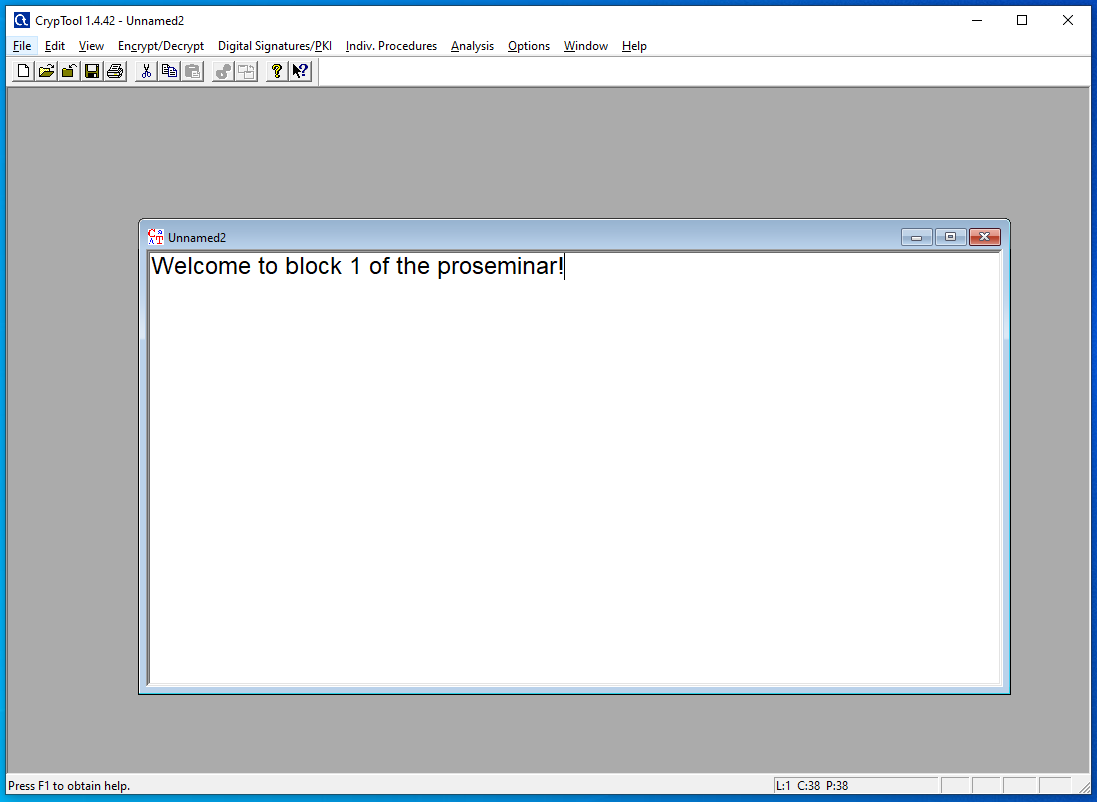
\includegraphics[scale=0.35]{figures/cryptool1.PNG}
    \caption{The code of this figure can be used when preparing your homework.}
    \label{fig:demo}
\end{figure}

\subsection{How to Include a Table}

A table can be included using the commands used to obtain Table \ref{tab:example}.

\begin{table}[ht]
    \centering
    \begin{tabular}{|c|c|c|}
    \hline
        Software & Assessment & Comments \\
        \hline
        Suite A & works well & internal use only \\
        \hline
        Suite B & freely usable & observe guidance document \\
        \hline
        Suite C & restricted & Requires compiler \\
        \hline 
    \end{tabular}
    \caption{Caption}
    \label{tab:example}
\end{table}

\subsection{How to List Data like Hexdumps}

Hexadecimal encoding provides a way to encode data in a machine and human-readable way. The code that has been used to generate Listing \ref{lst:example} can be used to include hex-data, including the one provided by \ctone{}. 
\begin{lstlisting}[style=plusStyle, caption={Example for how to include hex-data.},basicstyle=\tiny\ttfamily,label=lst:example]
50 63 D8 D0 D8 E4 FC F7 09 FB 1F 40 C1 99 E7 62 56 8A 20 77 B9 D6 F7 21 B3 61 F0 8D
96 AA 45 E3 A0 A5 11 97 58 17 2B 53 60 6D A3 2C A0 4C 2E 1F 5F 31 94 6A CC 09 28 8E
E0 0E 7C 23 2E 2F E3 E6 6A 02 AA D2 A7 41 80 6D AF 5D 72 63 0E AE A8 1F 3A 38 E3 91
74 56 B6 D7 59 C8 14 4B 0F C2 D8 9F 46 98 26 92 AF 5D 60 9E 5D AC 30 A1 DD 7A D1 95
49 AD 54 3C 93 B0 DF BC B2 57 83 AF F7 43 D8 98 0B 06 A4 6B 42 4C 8D 44 F4 7C BB B0
A6 B3 A2 7E 9C 11 D7 A6 98 23 EC 23 8E C8 AC FD 15 B0 2F 2B EC 49 25 B5 70 9C 0B D5
8A 24 5F 8C 7D 1A 32 E9 4C EF E7 B1 06 C7 D4 A2 C8 DA 01 15 99 E2 92 6B 0E DF 5B 36
15 2B 30 30 E0 5A A6 E0 80 2F 07 4F B4 4F 66 F8 17 A0 A3 72
\end{lstlisting}


\end{document}

